%  LaTeX support: latex@mdpi.com 
%  For support, please attach all files needed for compiling as well as the log file, and specify your operating system, LaTeX version, and LaTeX editor.

%=================================================================
\documentclass[gene,journal,article,submit,moreauthors,pdftex]{Definitions/mdpi} 
\usepackage{natbib}
\usepackage[colorinlistoftodos]{todonotes}
\newcounter{mycomment}
\newcommand{\mycomment}[2][]{%
% initials of the author (optional) + note in the margin
\refstepcounter{mycomment}%
{%
\setstretch{0.7}% spacing
\todo[color={red!100!green!33},size=\small]{%
\textbf{Comment [\uppercase{#1}\themycomment]:}~#2}%
}}
% For posting an early version of this manuscript as a preprint, you may use "preprints" as the journal and change "submit" to "accept". The document class line would be, e.g., \documentclass[preprints,article,accept,moreauthors,pdftex]{mdpi}. This is especially recommended for submission to arXiv, where line numbers should be removed before posting. For preprints.org, the editorial staff will make this change immediately prior to posting.

%--------------------
% Class Options:
%--------------------
%----------
% journal
%----------

%---------
% article
%---------
% The default type of manuscript is "article", but can be replaced by: 
% abstract, addendum, article, book, bookreview, briefreport, casereport, comment, commentary, communication, conferenceproceedings, correction, conferencereport, entry, expressionofconcern, extendedabstract, datadescriptor, editorial, essay, erratum, hypothesis, interestingimage, obituary, opinion, projectreport, reply, retraction, review, perspective, protocol, shortnote, studyprotocol, systematicreview, supfile, technicalnote, viewpoint, guidelines, registeredreport, tutorial
% supfile = supplementary materials

%----------
% submit
%----------
% The class option "submit" will be changed to "accept" by the Editorial Office when the paper is accepted. This will only make changes to the frontpage (e.g., the logo of the journal will get visible), the headings, and the copyright information. Also, line numbering will be removed. Journal info and pagination for accepted papers will also be assigned by the Editorial Office.

%------------------
% moreauthors
%------------------
% If there is only one author the class option oneauthor should be used. Otherwise use the class option moreauthors.

%---------
% pdftex
%---------
% The option pdftex is for use with pdfLaTeX. If eps figures are used, remove the option pdftex and use LaTeX and dvi2pdf.
%=================================================================
% MDPI internal commands
\firstpage{1} 
\makeatletter 
\setcounter{page}{\@firstpage} 
\makeatother
\pubvolume{1}
\issuenum{1}
\articlenumber{0}
\pubyear{2021}
\copyrightyear{2020}
%\externaleditor{Academic Editor: Firstname Lastname} % For journal Automation, please change Academic Editor to "Communicated by"
\datereceived{} 
\dateaccepted{} 
\datepublished{} 
\hreflink{https://doi.org/} % If needed use \linebreak
%------------------------------------------------------------------
% The following line should be uncommented if the LaTeX file is uploaded to arXiv.org
%\pdfoutput=1

%=================================================================
% Add packages and commands here. The following packages are loaded in our class file: fontenc, inputenc, calc, indentfirst, fancyhdr, graphicx, epstopdf, lastpage, ifthen, lineno, float, amsmath, setspace, enumitem, mathpazo, booktabs, titlesec, etoolbox, tabto, xcolor, soul, multirow, microtype, tikz, totcount, changepage, paracol, attrib, upgreek, cleveref, amsthm, hyphenat, natbib, hyperref, footmisc, url, geometry, newfloat, caption
\usepackage{hyperref}
\usepackage[utf8]{inputenc}
%=================================================================
%% Please use the following mathematics environments: Theorem, Lemma, Corollary, Proposition, Characterization, Property, Problem, Example, ExamplesandDefinitions, Hypothesis, Remark, Definition, Notation, Assumption
%% For proofs, please use the proof environment (the amsthm package is loaded by the MDPI class).

%=================================================================
% Full title of the paper (Capitalized)
\Title{A modelling strategy to improve cacao quality and productivity }

% MDPI internal command: Title for citation in the left column
\TitleCitation{Title}

% Author Orchid ID: enter ID or remove command
\newcommand{\orcidauthorA}{0000-0000-0000-000X} % Add \orcidA{} behind the author's name
%\newcommand{\orcidauthorB}{0000-0000-0000-000X} % Add \orcidB{} behind the author's name

% Authors, for the paper (add full first names)
\Author{Angela Romero V $^{1,\ddagger}$*\orcidA{}, Adriana Gallego $^{2}$ and Anyela V. Camargo R.$^{1, \ddagger}$}

% MDPI internal command: Authors, for metadata in PDF
\AuthorNames{Firstname Lastname, Firstname Lastname and Firstname Lastname}

% MDPI internal command: Authors, for citation in the left column
\AuthorCitation{Romero, A.; Gallego, A.; Camargo, A.}
% If this is a Chicago style journal: Lastname, Firstname, Firstname Lastname, and Firstname Lastname.

% Affiliations / Addresses (Add [1] after \address if there is only one affiliation.)
\address{$^{1}$ \quad The John Bingham Laboratory, NIAB, 93 Lawrence Weaver Road, Cambridge CB3 0LE, UK 1\\$^{2}$ \quad Grupo BIOS, Centro de Bioinformática y Biología Computacional de Colombia - BIOS, Manizales, Caldas, Colombia, South America. }%; e-mail@e-mail.com}

% Contact information of the corresponding author
\corres{Correspondence: angela.romerovergel@niab.com} %; Tel.: (optional; include country code; if there are multiple corresponding authors, add author initials) +xx-xxxx-xxx-xxxx (F.L.)}

% Current address and/or shared authorship
%\firstnote{Current address: Affiliation 3} 
\secondnote{These authors contributed equally to this work.}
% The commands \thirdnote{} till \eighthnote{} are available for further notes

%\simplesumm{} % Simple summary

%\conference{} % An extended version of a conference paper

% Abstract (Do not insert blank lines, i.e. \\) 
\abstract{Crop modelling can support agronomical decisions of crop production under a range of scenarios improving competitiveness. Cocoa production systems in Latin America has a high importance over social and economic development, facing  the fight against hunger and poverty. Although Colombian cocoa has the potential to be in the high value markets for fine flavour, it is still not widely produced as the lack of adoptions of technologies by the traditional farmers. They empirically harvest after 5 or 6 months after flowering date. However, cocoa fruits development can be considered as the result of a number of physiological and morphological processes that can be described by mathematical relationships even under uncontrolled environments. Thus, we parametrized the SIMPLE crop model \citep{Zao2019simple} to predict the best time for harvest cocoa fruits in Colombia. The results showed an RRMSE of 7.2\% for the yield prediction, while the simulated harvest date varied between +/- 2 to 20 days depending on the temperature variations of the year between regions. This crop model application contributed to understand and predict the phenology of cacao fruits the varieties ICS95 y CCN51, which is key to produce high quality cacao beans.  The aim of this study was developed a practical tool for farmers on cocoa fields to predict the best moment to harvest, using easily available data for crop modelling such as flowering date and weather variables (solar radiation, rain, and temperature). }

% Keywords
\keyword{ICS95; CCN51; thermal time, flowering date } 

%%%%%%%%%%%%%%%%%%%%%%%%%%%%%%%%%%%%%%%%%%
\begin{document}
%%%%%%%%%%%%%%%%%%%%%%%%%%%%%%%%%%%%%%%%%%
%\setcounter{section}{-1} %% Remove this when starting to work on the template.

\section{Introduction}
Cocoa ( \textit{Theobroma cacao }L. ) is an important worldwide perennial tropical crop endemic to the South American rainforests \citep{zuidema2005, motamayor2002, argout2011, Rodriguez2019}. Cacao plant member of the Malvaceae (formerly Sterculiaceae)  botanical family such as  cotton \textit{ Gossypium hirstium} \citep{Nix2017cotton} wich is modeled in SIMPLE model \citep{Zao2019simple}. Cocoa is grown for its fruits, known as cacao pods.  \citep{ Niemenak2010, suarez2021}. Only the 5\% of the world cocoa yield is desalinated for Fine-cocoa production due to the low productivity of  the traditional crop management \citep{argout2011}.  In Colombia, cocoa  is  traditionally  consumed  as  a  beverage. It is one of the crops promoted by the Colombian government in the social and agricultural development  programs aimed at favouring peace in post-conflict regions \citep{Rodriguez2019, Abbott2019}. This crop is grown by approximately 52.000 families \citep{Gutierrez2020} and 98\% of production being carried out by small and medium-sized producers \citep{Garcia2014, Escobar2020}. Colombia registered an increase of 3.750 tons in production in 2020 compared to the previous year \citep{lamos2020}. 

Although Colombian cocoa has the potential to be in the high value markets for fine flavour \citep{Escobar2020}, it is still not widely produced as the lack of adoptions of technologies by the traditional farmers. They empirically harvest after 5 or 6 months after flowering date, hence they ferment cocoa beans without considering the  quality of the seeds at the harvest time. This produce heterogeneous characteristics between each fermentation batch diminishing the quality of cocoa final product \citep{Escobar2021}. To identify the best moment to harvest is important to consider physiological responses affected by climate variables such as rain, solar radiation and wind.  Thus,  for cocoa in Colombia, physiological simulation models may be valuable to identify the best moment to harvest cocoa considering variable weather conditions, soil types and cultivar specifications. 

Crop models represent a quantitative assumption of plant growth depending on sunlight interception efficiency values and climate data supported by a large amount of empirical and ground data. \citep{Reynolds2018}. Physiological crop models have shown to be very useful tool for provided agronomical advices and improvements of the cropping systems of annual crops mainly. Recently crop modelling studies are focusing on  perennial crops  production \citep{zuidema2005, Zao2019simple, Bai2020, Romero2021}. However, the information reported  is be less than for annual crops due to the lack of field data available , relatively high research costs and the difficulties of accumulated errors in long-term simulations \citep{zuidema2005}. For cacao there  approaches  to predict yield mainly  using algorithms of machine learning \citep{lamos2020} and just one mechanistic model simulates physiological cocoa performance  "SUCROS-cocoa" \citep{zuidema2005}. This crop model calculates light interception, photosynthesis, maintenance respiration,
evapotranspiration, biomass production and cocoa yield. It can be parametrised having data on cocoa physiology and morphology \citep{zuidema2005}. However,  there is not specific cocoa physiology data available from small and medium-sized producers. Thus, we adapted the simple generic crop model (SIMPLE) that could be easily modified for any crop to simulate development, crop growth and yield using few parameters such as weather and cultivar specification \citep{Zao2019simple}.

In this paper, we present a physiological parametrization of SIMPLE crop model for cocoa to predict the best harvest time  and yield production. We used the SIMPLE crop model \citep{Zao2019simple} for three reasons: 1: That it is very comprehensively described in the original paper. 2: That the code was available in R for initial trials and 3: That it had already been successfully fitted to other perennial crops in south America. Overall, the model simulates crop development, growth and yield, and predict the maturation day when the fruit is ready to harvest. It includes 13 parameters ( daily weather data, irrigation, and soil and key dates) to specify a crop type, with four of these for cultivar characteristics easily available from farmer. Thus, this could be used as  tool for small farmers with the aim to improve the quality of cocoa to become more competitive in Fine-cocoa market.

\section{Materials and Methods}
\subsection{Floral Phenology of Cocoa }
Normally the phenological stages in cocoa are  divided in two main phases: vegetative and reproductive. In the SIMPLE model we simulate the reproductive phase (fig. \ref{fig:pheno}, a) described by the floral phenology from the date of inflorescence emergence (BBCH scale 5) (fig. \ref{fig:pheno},b ) to predict the date of ripening of fruit and seed (BBCH 8) (fig. \ref{fig:pheno},c ) \citep{Niemenak2010} . In the Andean region the reproductive phase is cyclically fulfilled during two annual cycles passing by the following phases: inflorescence emergence, flowering, pollination, fruit development and harvest. Therefore, for modelling parametrization the crop cycle of cocoa as perennial plant does not start at the plantation date such as annual crops systems. Instead  the start point of the cocoa crop cycle to model is the inflorescence emergence date (fig. \ref{fig:pheno},b). Consequently , the growth period of the fruit can varied from  110 to 150  daa (days after anthesis) \citep{lopez2018} when cacao fruits reaches the physiological maturity, but it can be harvested at 170 days daa \citep{Niemenak2010} for quality purposes.

Cocoa is a cauliflorous plant, which means that flowers grow on the trunk and branches. In Colombia cocoa trees usually produce flowers throughout the year. Cocoa trees produces with up to 10000 flowers per tree each year, which the 50 \%  do not develop into ripe fruits according to Fedecacao reports. The flower takes 30 days passing by 12 micro-stages from meristem development (stages 1to 6) to the fully developed flower (Stages 7 to 12) \citep{swanson2005} when it is ready to be pollinated. The opening of flowers or anthesis  occurs over a 12-hour period during the night and it is synchronised between the groups of mature flowers \citep{Niemenak2010}. However, the live of a flower can last approximately 1 day after the opening falling form the trunk if it is unfertilised \citep{cheesman1927, Niemenak2010}.

Subsequentially, after anthesis the fruit growths by approximately 150 days until the maturation, mucilage. Therefore, the complete maturation process of the fruit, from the pollination to fully mature fruit, takes 160- 210 days \citep{berry1994}. The accumulation of lipids, storage proteins and anthocyanin starts about 85 days after pollination when fruits have an active metabolism and seeds   moisture content decreases up to 30\% \citep{Lehrian1980, Niemenak2010}. During this phase the quality of cocoa seeds is defined.


\begin{figure}[h!]
	\centering
	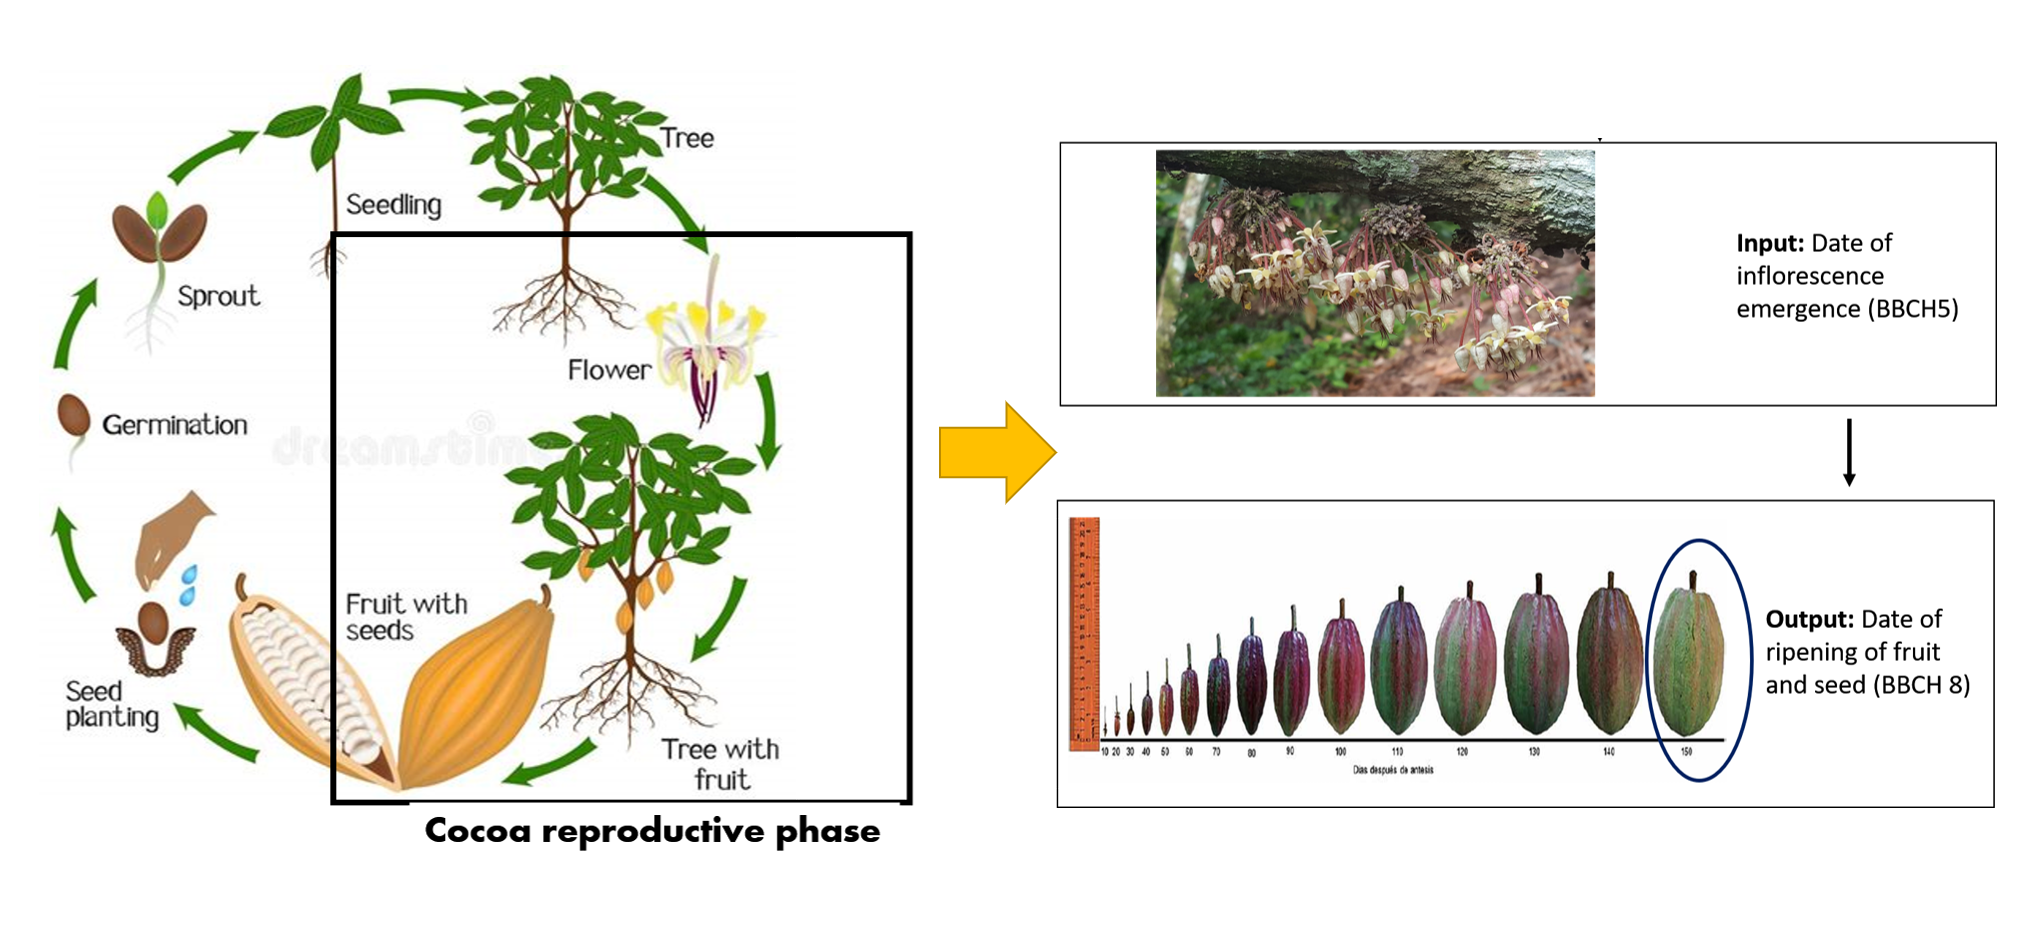
\includegraphics[scale=0.4]{images/phenology.png}\\
	\caption{\footnotesize {Phenology of cocoa in Colombia for crop modelling.\\}} 
	\footnotesize{Credits: Taken from from Dreamstime.com, phys.org \citep{toledo2021} and \cite{lopez2018}}
	\label{fig:pheno}
\end{figure}



\subsection{Test site and yield production }
Cacao is cultivated in 30 states out of 32 from the total Colombian territory with about 147,000 ha \citep{Meza2021}. Cocoa fields studied were located in Saravena (Arauca), Rionegro (Santander), Cali (Valle del Cauca), Apartado (Antioquia) and Manizalez (Caldas) (Fig.\ref{fig:yield}, b). We considered 112 parcels data from Fedecacao reports. Each parcel data contained age of crop, density of planting, yield, number of fruits harvested, flowering date, harvest date.   Acording to personal comunication from framers the biggest flowering occurs in September and January to harvest in March and July. However, the data reported showed that this flowering and pod productions are not constant for all the regions.  Cali and Caldas presented the lowest production. However, the pod harvest in Caldas increased in May and from October to December, and decreased from January to March.  Meanwhile, Arauca and Apartado reported the highest yield in the months January, July, November and December. Santander has picks of production in March, May and September (Fig.\ref{fig:yield}, a).

\begin{figure}[h]
	\centering
	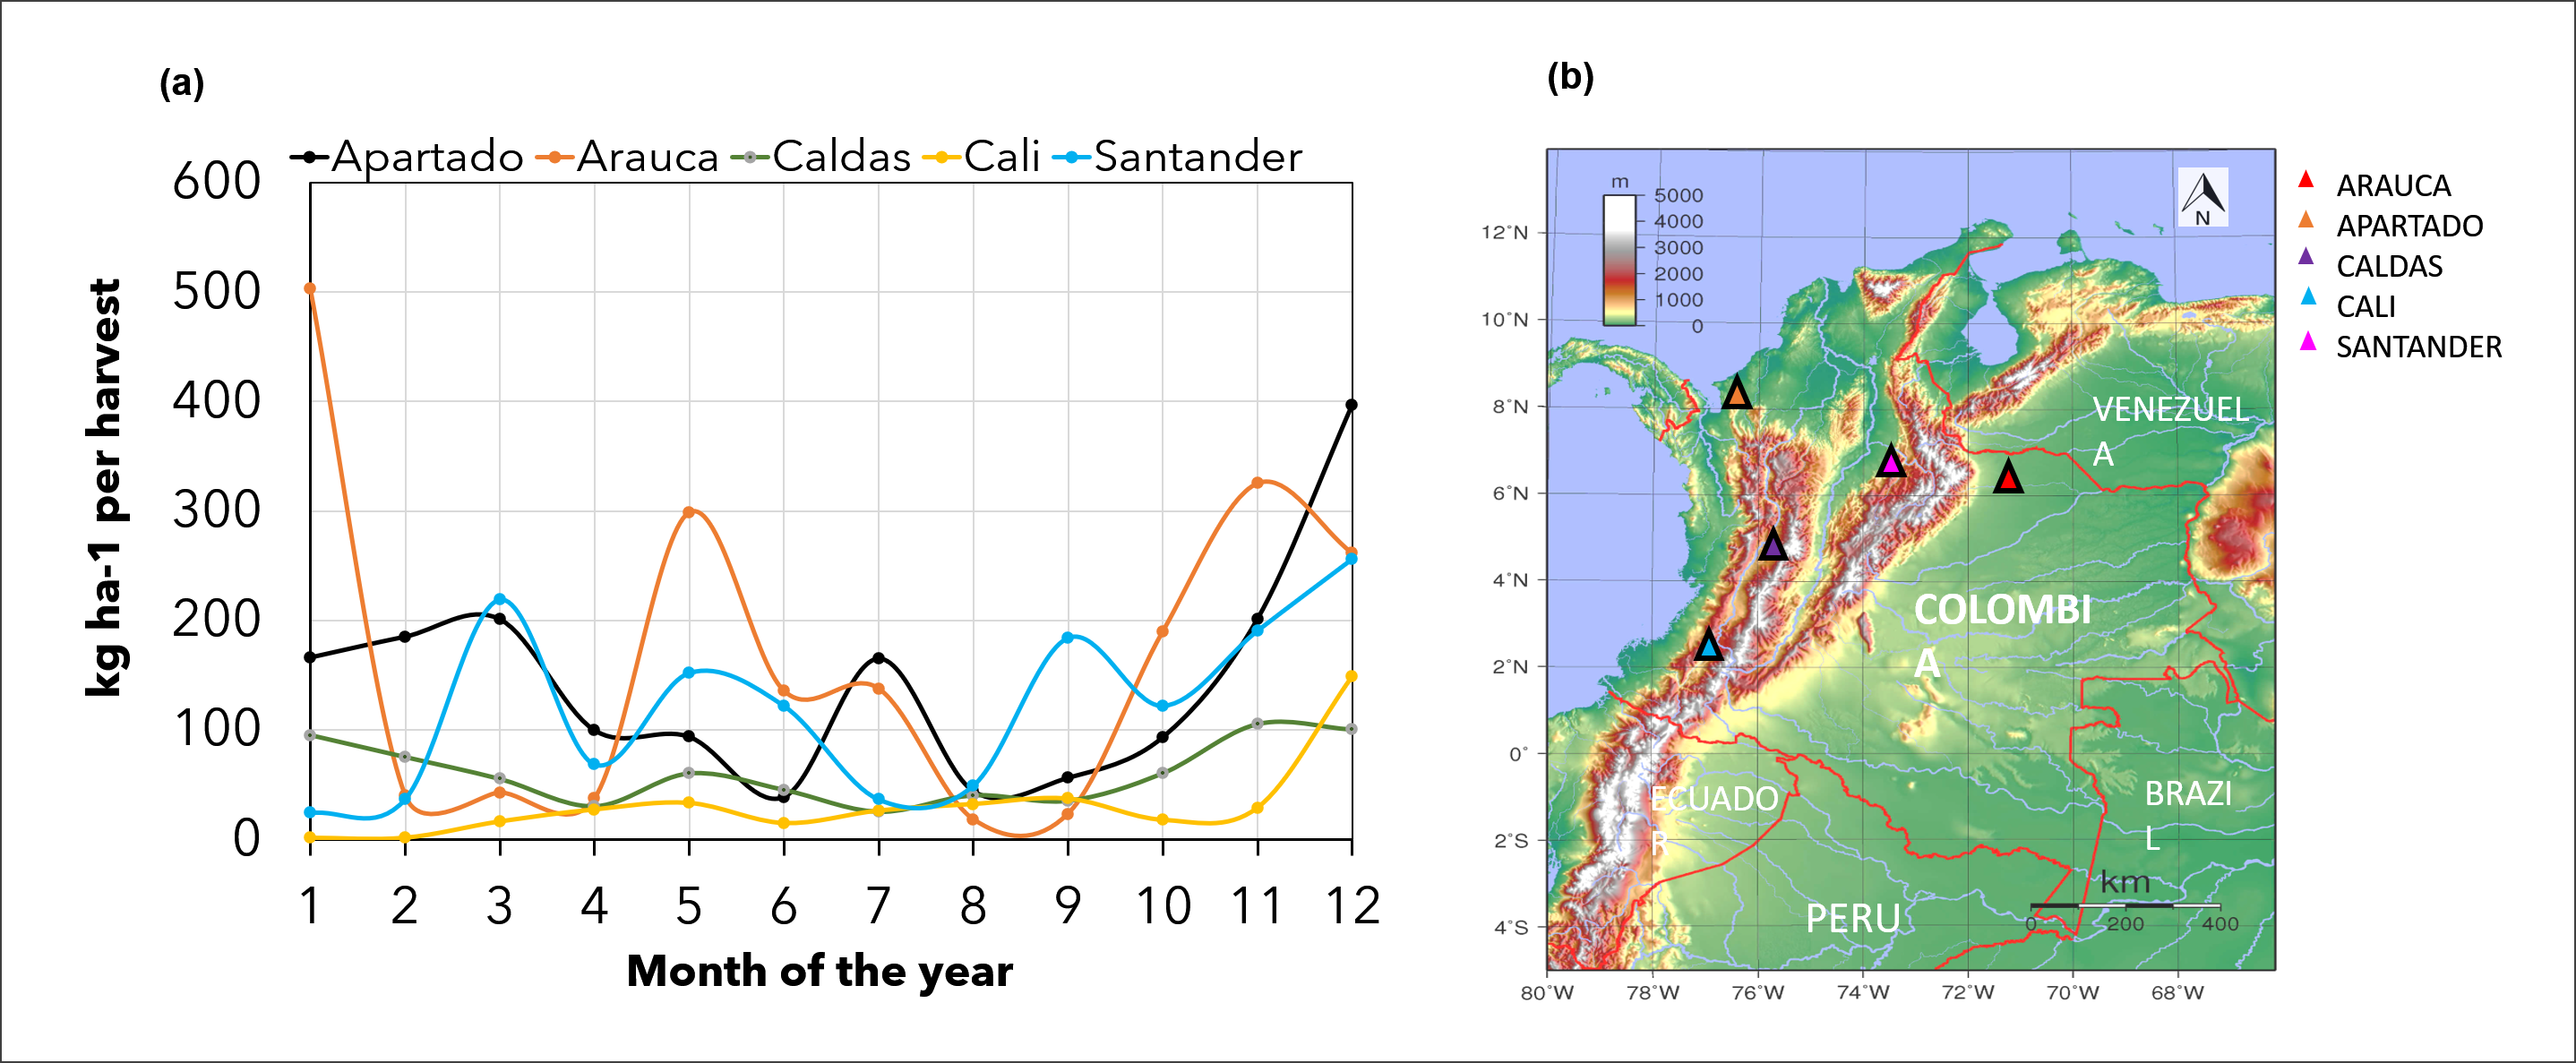
\includegraphics[scale=0.3]{images/map.png}\\
	\caption{\footnotesize {Cocoa production characterization of cocoa for five locations\\}}
	\label{fig:yield}
\end{figure}
\newpage

\subsection{Weather conditions}
\begin{figure}[h!]
	\centering
	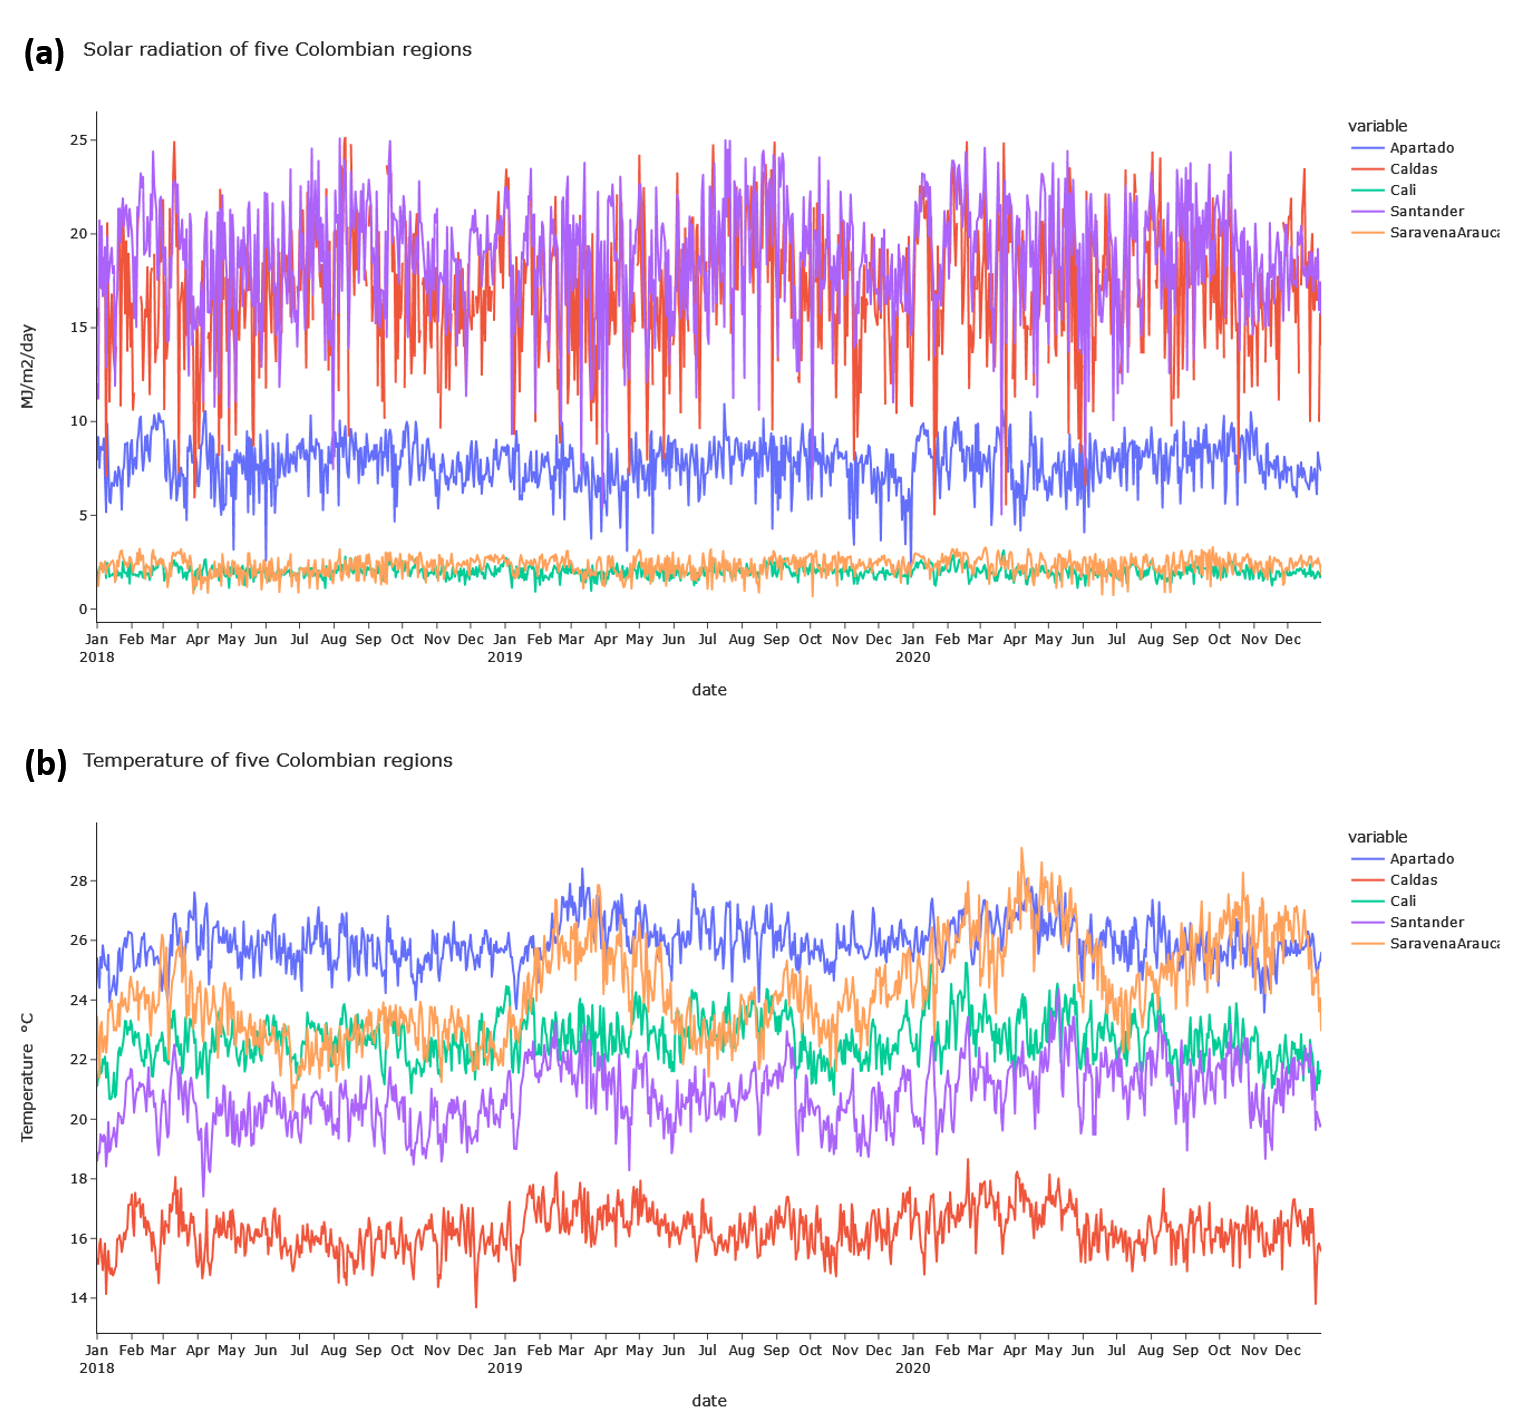
\includegraphics[scale=0.4]{images/clima.png}
	\caption{\footnotesize {Colombian weather conditions. \\}}	
	\label{fig:temp}
	{\footnotesize (a), available photosynthetic solar radiation (PAR). (b), Daily average temperature  (c), Precipitation and relative humidity per month}
\end{figure}
\newpage

Solar radiation (PAR), temperature, precipitation ant relative humidity was studied from 2018 to 2020 (Fig.\ref{fig:temp}). Santander and Caldas had the biggest variability and the maximum of solar radiation values over 20 MJ m$^{2}$day$^{-1}$. In contrast , Cali and Arauca presented the lowest values of PAR below 5 MJ m$^{2}$day$^{-1}$. (Fig.\ref{fig:temp}, a).  Even though, Cali and Santander had contrasting PAR conditions, they regions presented  have similar temperature during 2020 (Fig.\ref{fig:temp}, b). The temperature ranges from 16 to 28 $^\circ$C and it is relatively constant for each region. However, Arauca presented the biggest variability with hotter months during the first half of the year 2019 and 2020.  Apartado was found as the hottest region studied with 26 $^\circ$C and Caldas as the coldest site with 18 $^\circ$C.  Precipitation in Colombia is presented in two seasons per year from February to April and from October to November, while the relative humidity remain constant over 80\% (Fig.\ref{fig:temp},c). In general, the coldest regions tested (Caldas and Santander) had the maximun values of solar radiation available for photosynthesis. 





\subsection{Thermal time for pod harvest date identification}
It is required to model crop growth  considering the cocoa base temperature (T$_{b}$), at which the plant development stops \citep{Ritchie1991}. This characterization was conducted for the five regions counted 180 days (6 months) after flowering, as farmers used to harvest by calendar days. Characterizing the thermal time the models predicts the maturation day to harvest the cocoa can vary depending on temperature variations. Thermal time (degree days) was calculated  from the flowering date to the pod harvest  using the ecuation \ref{equ:tem}. Where tt is the cumulative sum of the daily temperature (T$_{i}$) and T$_{b}$ for cocoa is 10$^\circ$C according to \cite{lahive2019}.

\begin{equation}
Thermal~time~(tt) = \left\lbrace\begin{array}{c} \sum_{i=1}^{n} T_{i} - T_{b} \\
\vspace{0.2cm}\\ 
0,\hspace{0.2cm} Flowering~date\end{array}\right.
\label{equ:tem}
\end{equation}


\subsection{Model Calibration}

Calibration of crop models are conducted typically for particular cultivars and require site specific inputs for weather \citep{Crout20142}. The procedure for the SIMPLE model \citep{Zao2019simple} calibration  was a sequential process of modifying physiological variables specific for cocoa in the inputs files and  adding the appropriate files of weather for each region tested. In the SIMPLE model has seven input files where new cocoa crop data should be provided. Files in the list below can be edited to define the features of the new cultivars or experiments. Cocoa crop has not been simulated with SIMPLE model, hence consider previous cocoa studies, values such as leaf area index (LAI) \citep{Agele2016} and Harvest index (HI) \citep{Quintana2015} where modified. Radiation Use Efficiency (RUE) was calibrate according to the perennial crops  (banana and cotton) that had been calibrated previously in SIMPLE model \citep{Zao2019simple} with a RUE of 0.8 and 0.85 respectively. As cocoa trees are under shadow the RUE was lower with values between 0.7 and 0.5 g MJ$^{\mathbf{-1}}$ m$^{2}$ (table \ref{tab:reparam}).
Once the physiological parameters were calibrated to the  simulated yields for cocoa were reasonably close to the observed yield. 23 flowering dates from 12-July-2019 to 23-June-2020 were introduced in the treatment file, running the program and saving the results.  

\begin{enumerate}
	\item Input/Simulation Management.csv
	\item Input/Species parameter.csv
	\item Input/Cultivar.csv
	\item Input/Treatment.csv	
	\item Input/Soil.csv
	\item Observation/Obsdummy crop Exp name.csv	
	\item Weather/dummy weather.WTH
\end{enumerate}


\subsection{Inputs and parameters}
Input variables required to run SIMPLE model for cocoa include the flowering date and daily weather of solar radiation (SRAD), maximum and minimum temperature (TMAX, TMIN) and rain. Weather data as csv file was  downloaded from the POWER Data Access Viewer \citep{nasapower} from January 01 2018 to December 31 2020 for four locations in Colombia (Cali, Rionegro -Santander, Apartado - Antioquia, Saravena Arauca). The csv file had to be transformed to .WHT file using R 1.4 version \citep{Rstudio2020}. 

There were three parameters varied by region (table \ref{tab:reparam}) thermal time required for pod harvest after the flowering date (Tsum) , the Radiation use efficiency (RUE) and yield observed on field. Physiological parameters in table \ref{tab:Treaparam} are  common  for all the regions studied. These parameter were calibrate for cultivars ICS95 and CCN51 considering a range of time of 200 days (DAP) from flowering date to harvest day, even thought farmers collect the pod at 180 DAP. Heat and water stress parameters were not considered.


\begin{table}[h!]	
	\caption {\footnotesize {Cocoa crop parameter values used per region.}}
	\label{tab:reparam} 
	\centering
	\begin{small}
		\begin{tabular}{l c c c }
			\hline
			{\bf Region }&{\bf Tsum }&{\bf RUE}&{\bf Yield$^{*}$}\\
			\hline
			Apartado   & 2906 & 0.6 & 3378  \\
			Arauca   & 2764 & 0.7 & 3981  \\
			Santander & 2016 &0.6 & 2687 \\
			Cali   & 1912 & 0.5 & 1900  \\
			Caldas   & 1192 & 0.6 & 740  \\
			\hline
		\end{tabular} \\
		{\footnotesize RUE Radiation use efficiency (above ground only and without respiration)g MJ$^{\mathbf{-1}}$ m$^{\mathbf{2}}$\\$^{*}$ Yield observed kg ha$^{\mathsf{-1}}$ per year. } 
	\end{small}
\end{table}


\begin{table}[h!]	
	\caption {\footnotesize {Parameter values used to run SIMPLEcocoa model.}}
	\centering
	\label{tab:Treaparam} 
	\begin{small}
		\begin{tabular}{{l l l}}
			\hline
			{\bf File }&{\bf Variable name }&{\bf Value}\\
			\hline
			&SoilName & Loamy sand4\\
			&InitialFsolar & 0.01\\
			Treatment&Weather & KOKO (.WTH file name)\\
			&CO$_{2}$ & 400 ppm\\
			&SowingDate &Flowering date\\
			\hline
			&Crop cycle DAP & 200 days\\
			&LAI & 1.8 \\
			Observation&FSolar& 0.70\\
			&Biomass & 40kg dry mass per plant\\
			\hline
			&Harvest index & 0.3\\
			Cultivar&150A & 680 $^\circ$C day \\
			&150B & 680 $^\circ$C day \\
			\hline
			&Tbase & 10$^\circ$C\\
			&Topti & 26$^\circ$C \\
			Species&MaxT & 35$^\circ$C \\
			&ExtremeT & 40$^\circ$C  \\
			&CO$_{2}$RUE & 0.09$^\circ$C  \\			
			&S-water & 0 ARID index \\
			\hline			
		\end{tabular} \\ 
	\end{small}
	{\footnotesize S-water is associated drought stress evaluations ranging from 0 (no water shortage) to 1 (extreme water shortage) \cite{Zao2019simple} }
\end{table}
\newpage


\subsection{Evaluation of model performance}

The SIMPLE model performance was evaluated by comparing simulated values cocoa yield with those reported by Fedecacao from cocoa plantations, using the statistical indice of relative root mean square error (RRMSE) (Equ. \ref{equ:RMSE}) \citep{Zao2019simple, Bai2020}. 


\begin{equation}
RMSE= \sqrt{\frac{1}{n}  \sum_{i=1}^{n} (Y_{i}-X_{i})^{2} } 
\label{equ:RMSE}
\end{equation}



\section{Results}

\subsection{Thermal time }
Thermal time characterization is shown in figure \ref{fig:ttbox}. It showed differences per region as was expected following the tendencies of the temperature per region (fig. \ref{fig:temp},c). Apartado and Arauca had the highest temperatures hence, the highest thermal time values with 2909 and 2764 days$^\circ$C  respectively. Caldas had the lowest values with 1173 days$^\circ$C. Meanwhile, Cali and Santander presented similar thermal time around 2000 $^\circ$C (table \ref{tab:reparam}). The accumulated temperature during the pod development (fig.\ref{fig:ttbox}) depends on the region where cocoa is cultivated and the variety planted. Thermal time values are also proportional to the yield reported on field (table \ref{tab:reparam}).\\

\begin{figure}[h!]
	\centering
	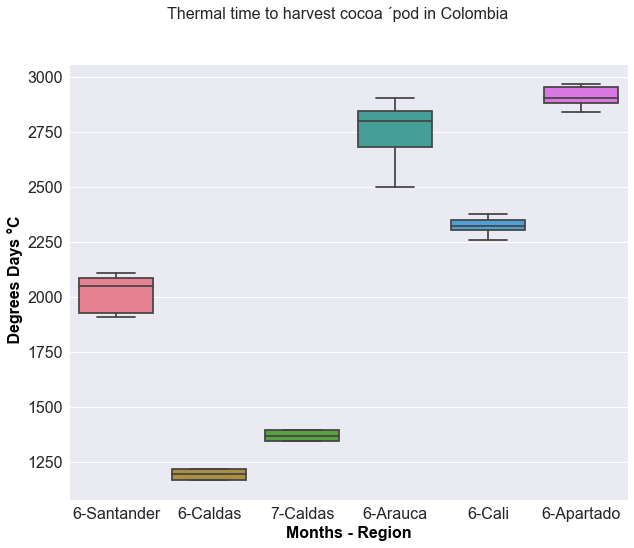
\includegraphics[scale=0.3]{images/ttbbox.png}\\
	\caption{\footnotesize {Coaoa yield and thermal time characterization.\\}}
	\label{fig:ttbox}
\end{figure}


\subsection{Weather effects over flowering time }

Figure \ref{fig:heat} shows the pearson correlation to study the weather data of the flowering time over the months of flowering  (monthF), month of harvest (monthH) and their final yield (fruit\_kg) . The results showed that thermal time with T$_{b}$ (ttb), temperature minimum and maximum (TMIN and TMAX) and Dew Frost Point at 2 meters (T2MDEW) are positive related. The wind (WS2M) is clear correlated with ttb. However, less clear correlations were found of monthF  with T2MDEW, relative humidity (RH), WS2M and rain.  

\begin{figure}[h!]
	\centering
	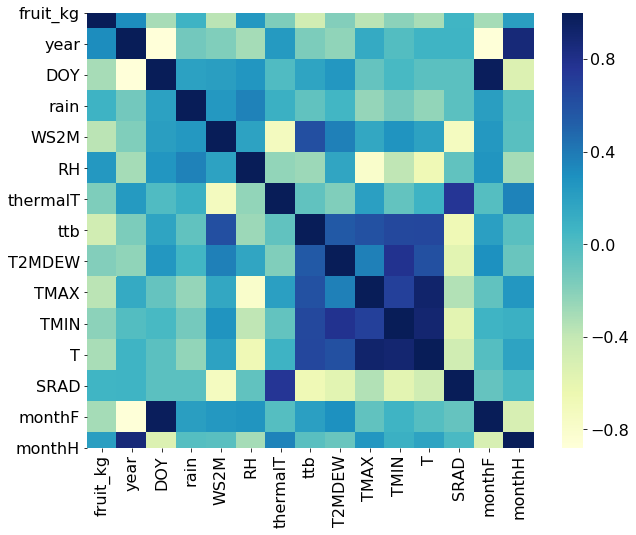
\includegraphics[scale=0.35]{images/heatm.png}\\
	\caption{\footnotesize {Pearson correlation among weather variables and flowering dates all locations. \\}}
	\label{fig:heat} 
\end{figure}

\subsection{Model validation}
The cocoa yield simulation (kg ha$^{-1}$ per year) was validated using observed data (table \ref{tab:reparam}) showing a final RRMSE of 7.2\% (fig. \ref{fig:m1}, a). Individual errors per region are presented in table \ref{tab:error}, where the best fit simulation model was for yield prediction in Apartado and the highest error was calculated for Caldas crops.  The model responded to the variations of temperature and solar radiation. Therefore, the highest  yield values simulated were obtained for Arauca over 4000 kg ha$^{-1}$, followed by Apartado Santander with yields over 2000 kg ha$^{-1}$.  The lowest yield was simulated for Caldas region with less of 1000 kg ha$^{-1}$ . Final yield in the model was is calculated as the product of biomass of aerial part and harvest index (HI) \citep{Zao2019simple, Amir1991}, where the HI is similar to the CropSyst \citep{STOCKLE2003} and AquaCrop \cite{Steduto2009}. 

Therefore, biomass production of the aerial part of the plant was simulated per region (fig. \ref{fig:m1}, b) as biomass-rate which is the daily biomass growth rate.  As for cocoa simulation we did not consider water and heat stress variables, in this research biomass simulation is affected by the solar radiation, RUE, daily temperature, atmospheric CO$_{2}$ concentration (ppm) and the fraction of solar radiation intercepted by a tree of cocoa during the fruit development (fSolar) (fig. \ref{fig:m1}, c). Due to the lack of this kind of data from fields, the comparison was not possible with observed data of biomass production through the crop cycle. However, the biomass simulation also responded proportionally with the yield production. Biomass of cocoa fruits simulated include all the parts that compound  the pod when they are fresh. Therefore, these this information may be of interest to farmers to predict pod fresh mass. 

The figure \ref{fig:m1}, c the fSolar was simulated thought the fruit development resulting that crops in  all regions reached the maximun fSolar at 0.94, except Caldas where crops reached 0.76.  Apartado and Arauca reached faster this fSolar-max. These high values of solar radiation intercepted for photosynthesis, lasted differently depending on the region and their solar radiation (Fig.\ref{fig:temp}, a) : Apartado 66 days  from  69 to 135 days after flowering (daf),  Arauca 61 days from 72 to 133 daf, Cali 38 days from 83 to 121 daf,  Santander 24 days from 92 to 116 daf and Caldas 2 days at 125 daf. fSolar declined in the interception of solar radiation until the pod harvest day. 

\begin{figure}[h!]
	\centering
	\includegraphics[scale=0.4]{images/outmodel.png}
	\caption{\footnotesize {SIMPLE model output for cocoa in Colombia.\\ }} 
	\label{fig:m1}
\end{figure}

\begin{table}[h!]	
	\caption {\footnotesize {Summary of relative root mean square error RMSE for the predicted cocoa yield using SIMPLE model.}}
	\label{tab:error} 
	\centering
	\begin{small}
		\begin{tabular}{l c c c c c c}
			\hline
			{\bf Region }&{\bf Apartado }&{\bf Arauca}&{\bf Santander}&{\bf Cali}&{\bf Caldas}&{\bf Overal}\\
			\hline
			RMMSE \%  & 3 & 6.05 & 10.06&8.5&14.90&7.2 \\
			\hline
		\end{tabular} \\
	\end{small}
\end{table}


\subsection{Prediction of the pod harvest day }
These result demonstrated that the traditional way to harvest always at 180 daf is not having account physiological and environmental conditions that can be affecting the pod development and maturation.
Figure \ref{fig:dayH} present that observe day of harvest or maturity day is 180 daf independently of the region. All the regions except Santander, presented the earliest harvest when the flowering date was between December and February. The fruit can be ready to harvest depending of the enviromental condition per region. Thus, when the fruit development was simulated the maturity day in Cali and Caldas were from 3 to 12 and 4 to 23 days before 180 daf (Fig. \ref{fig:dayH}, c and f respectively). Apartado presented the most similar predicted dates of harvest to 180 daf with 170 to 182 daf  (Fig. \ref{fig:dayH}, d). The pod may be harvest in Arauca (Fig.\ref{fig:dayH}, b)  between 165 and 193 daf, Santander (Fig.\ref{fig:dayH}, a) between 165 and 183 daf, ten days less than in Arauca for the same months of flowering of July and August of 2019 . 
 
\begin{figure}[h!]
	\centering
	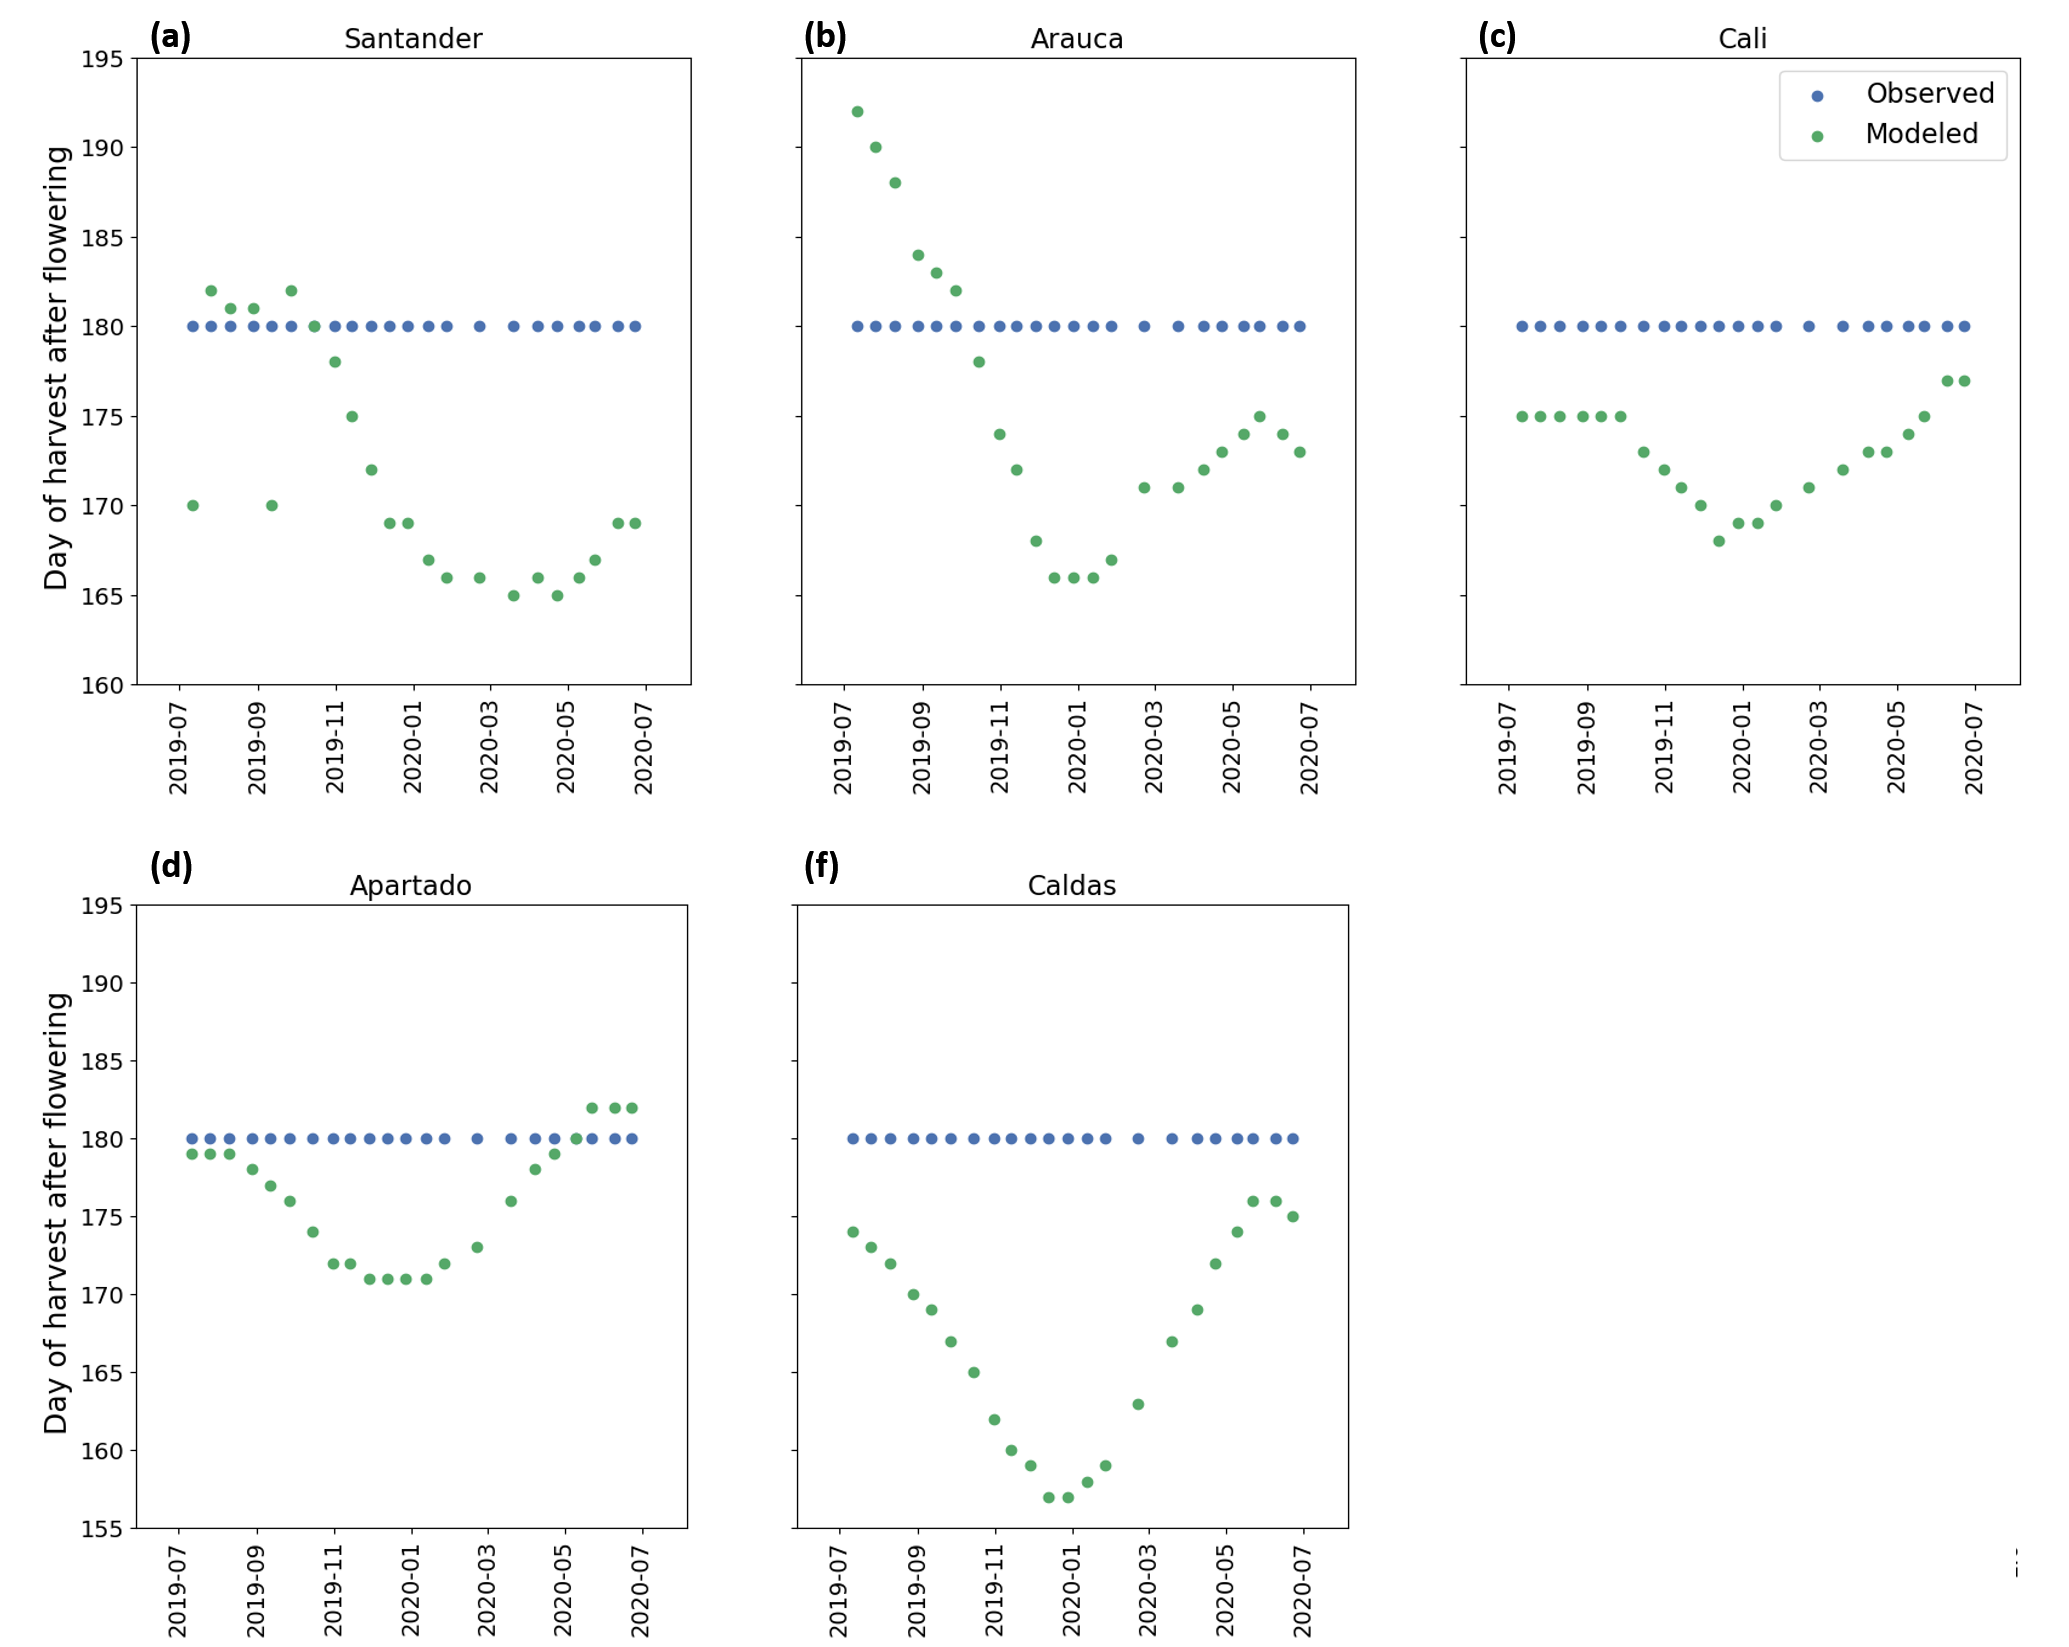
\includegraphics[scale=0.4]{images/RegionHarvest2.png}
	\caption{\footnotesize {Day of harvest cocoa simulation\\ }} 
	\label{fig:dayH}
\end{figure}.
\newpage


%%%%%%%%%%%%%%%%%%%%%%%%%%%%%%%%%%%%%%%%%%

\section{Discussion}
Authors should discuss the results and how they can be interpreted from the perspective of previous studies and of the working hypotheses. The findings and their implications should be discussed in the broadest context possible. Future research directions may also be highlighted.

This study presents a new approach of SIMPLE model calibration for cocoa as tropical crop in South America for five environments.

The optimum temperature for photosynthesis in cacao has
been reported to be between 31 °C and 33 °C (Balasimha et al.
1991) and 33 °C–35 °C (Yapp 1992). Sena Gomes and
Kozlowski (1987) reported a decrease in gs over the range
18.7 °C to 27.2 °C and an increase at temperatures above this,
most likely to enhance cooling at higher temperatures.
However, the opposite effect was described by Raja Harun
and Hardwick (1988a). In this study, gs and transpiration (E)
increased within the range of 20 °C–30 °C. In field-grown
cacao in India, photosynthetic rate declined as mean monthly
temperature increased above 34 °C during the dry season
(Balasimha et al. 1991). \cite{lahive2019}
\textcolor{red}{this section on going to organize}

Evaluating the level of knowledge of producers regarding cocoa crop management, the harvest was in the group of activities that presented the lowest level of knowledge on the part of the producers according to the general averages \citep{Gutierrez2020}. 

\subsection{Weather Effects}
Wind can affect the availability of tiny flies pollinators from Diptera order and from the families of of the biting midges \textit{Ceratopogonidae},  genus  \textit{Forcipomyia} \citep{Saunders1959, kaufmann1975, sotomayor2020} to reach the cocoa flowers. However, wind is not included in the SIMPLE model as an input as cocoa crop has not been simulated with this model before. Flower opening is very well synchronised between the cohorts of mature flowers opening each night. The flowers open at almost exactly the same time and rate, irrespective of their position on the trunk. Unfertilised flowers abscise from the trunk approximately 1 day after flower opening  \citep{Niemenak2010}.  In a preliminary analysis of Santanter data, We found that the number of successful flowers pollinated to produce final yield can be affected mostly by the rain, TMAX and wind (fig.\ref{fig:heat}).

\subsection{App development and future challenges }
The original code of SIMPLE model of \citep{Zao2019simple} was modified to make easy the implementation of this cocoa model as and app to be used in smartphones and desktops by farmers in Colombia. Therefore, the new version for cocoa crops simulation will be used to predict yield, date of harvest and biomass production, inserting only the date of flowering and region. The app development is on charge of Grupo BIOS to be deliver to farmers in Caldas initially at the end of 2021. 
This research presented and initial crop calibration that can be improved with further studies, including effects over the pod production by diseases, nutritional diffidences and abiotic stresses. The future challenge will be that traditional farmers start to harvest more aware of the environmental effects over their crops. It will be necessary that they engage growers with adapt founding from scientific studies. Moreover, It will be required the help of entrepreneurs, researchers, academics and non-specialized communities to transfers the knowledge to cocoa growers.
%%%%%%%%%%%%%%%%%%%%%%%%%%%%%%%%%%%%%%%%%%
\section{Conclusions}
Based on principles of crop physiology this  generic crop model , which was developed with relatively few equations and parameters was fitted for cocoa fruit growth. The SIMPLE model worked well for cocoa yield prediction and to demonstrate that the moment to harvest the cocoa pod is affected by the weather variations over the physiology of the trees.

\acknowledgments{The authors wish to thank to Grupo BIOS and Fedecacao for facilitated the data from cocoa fields. In this section you can acknowledge any support given which is not covered by the author contribution or funding sections. This may include administrative and technical support, or donations in kind (e.g., materials used for experiments).}

\conflictsofinterest{The authors declare no conflict of interest.}



%%%%%%%%%%%%%%%%%%%%%%%%%%%%%%%%%%%%%%%%%%
\end{paracol}
%%%%%%%%%%%%%%%%%%%%%%%%%%%%%%%%%%%%%%%%%%
% To add notes in main text, please use \endnote{} and un-comment the codes below.
%\begin{adjustwidth}{-5.0cm}{0cm}
%\printendnotes[custom]
%\end{adjustwidth}
%%%%%%%%%%%%%%%%%%%%%%%%%%%%%%%%%%%%%%%%%%
\reftitle{References}

% Please provide either the correct journal abbreviation (e.g. according to the “List of Title Word Abbreviations” http://www.issn.org/services/online-services/access-to-the-ltwa/) or the full name of the journal.
% Citations and References in Supplementary files are permitted provided that they also appear in the reference list here. 

%=====================================
% References, variant A: external bibliography
%=====================================
\externalbibliography{yes}
\bibliography{kokobib}
\end{document}